\let\textcircled=\pgftextcircled
\chapter{Context and Dataflow Diagrams}

\section{Context Diagram}

\vspace{2cm}
\begin{figure}[H]
\caption{Context Diagram}
\vspace{1cm}
\centering
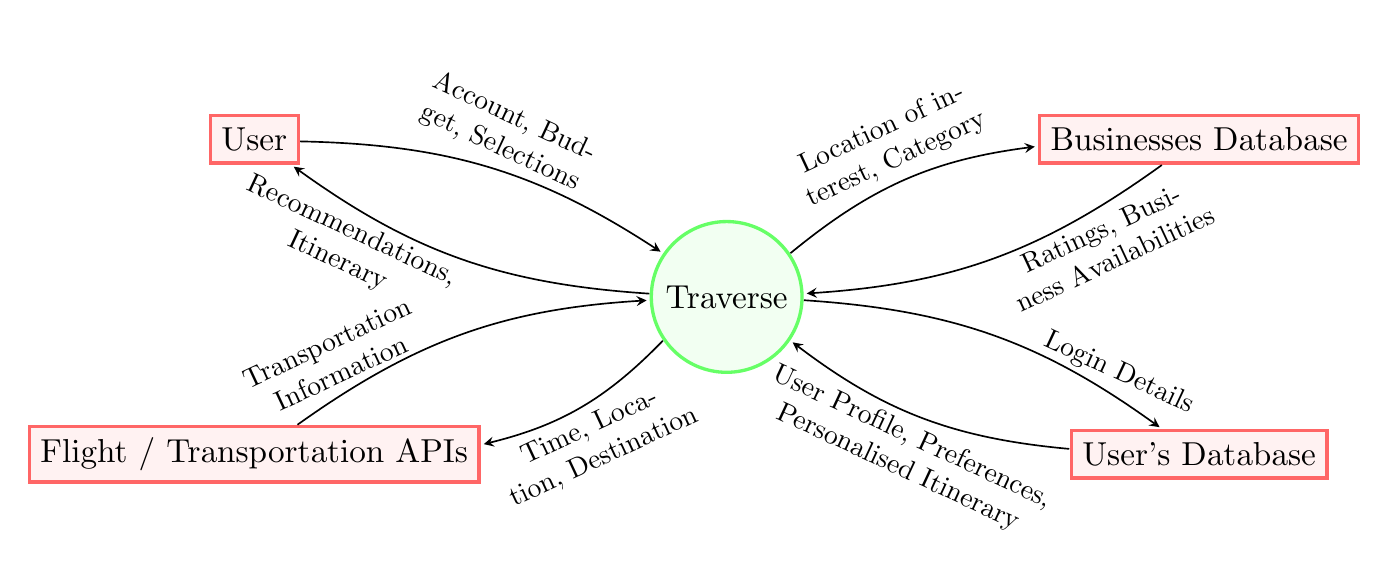
\begin{tikzpicture}[
roundnode/.style={circle, scale = 1.2, draw=green!60, fill=green!5, very thick, minimum size=7mm},
squarednode/.style={rectangle, scale = 1.2, draw=red!60, fill=red!5, very thick, minimum size=5mm},
to/.style={->,>=stealth,shorten >=1pt,semithick},
]
%nodes
\node[squarednode](e1) at (-6, 2) {User};
\node[roundnode](p) at (0,0) {Traverse};
\node[squarednode](e2) at (6, 2) {Businesses Database};
\node[squarednode](e3) at (-6, -2) {Flight / Transportation APIs};
\node[squarednode](e4) at (6, -2) {User's Database};
%connections
\draw[to] (e1) to [bend left = 16] node[align=center, text width = 4cm, above = 0cm, rotate=-25] {Account, Budget, Selections}(p);
\draw[to] (p) to [bend left = 16] node[align=center,text width = 4cm, pos=0.8, below = 0cm, rotate=-25] {Recommendations, Itinerary}(e1);
\draw[to] (p) to [bend left = 16] node[align=center,text width = 4cm, midway, above = 0cm, rotate=25] {Location of interest, Category}(e2);
\draw[to] (e2) to [bend left = 16] node[align=center,text width = 4cm, pos=0.2, below = 0cm, rotate=25] {Ratings, Business Availabilities}(p);
\draw[to] (e3) to [bend left = 16] node[align=center, text width = 4cm, above = 0cm, pos=0.15, rotate=25] {Transportation Information}(p);
\draw[to] (p) to [bend left = 16] node[align=center,text width = 4cm, midway, below = 0cm, rotate=25] {Time, Location, Destination}(e3);
\draw[to] (p) to [bend left = 16] node[align=center,text width = 4cm, pos=0.85, above = 0cm, rotate=-25] {Login Details}(e4);
\draw[to] (e4) to [bend left = 16] node[align=center,text width = 4cm, midway, below = 0cm, rotate=-25] {User Profile, Preferences, Personalised Itinerary}(p);
\end{tikzpicture}
\end{figure}

\section{Data Flow Diagram - Core Functionality}
\begin{figure}[H]
\caption{Data Flow Diagram - Core Functionality}
\vspace{0.3cm}
\centering
\begin{tikzpicture}[node distance = 2.5cm,
process/.style={circle, scale = 0.8, align=center, text width = 2cm, draw=green!60, fill=green!5, very thick, minimum size=7mm},
entity/.style={rectangle, scale = 1.2, align=center, text width = 2cm, draw=red!60, fill=red!5, very thick, minimum size=5mm},
path/.style={->,>=stealth,shorten >=1pt,semithick},
]

\tikzset{
  pics/datastore/.style args={#1,#2, #3}{
     code={
	     \draw [draw=blue!60] (0,0) -- (3,0) -- (3,1) -- (0, 1);
	     \node[#3] (#1) at (1.5,0.5) {#2};
     }
  }
}

%Nodes
\node [entity] (user) {User};
\node [process] (login) [below left = of user]{Login};
\node [process] (signup) [below right = of user]{Signup};
\node [process] (ansqs) [below = of signup, xshift=1cm]{Answer Preference Questions};
\draw (-1.5, -6) pic{datastore={ud1, User Database, black}};
\node [process] (loadint) [below = of login, xshift= -1cm]{Load Itinerary};
\node [process] (mlig) [below = of ud1]{Machine Learning Itinerary Generation};
\node [process] (conf) [below = of mlig]{Confirm Booking};
\node [entity, yshift= 0cm, xshift = 0.7cm] (user1) [below = of conf]{User};
\draw (3.5, -11) pic{datastore={ft1, Transport APIs, black}};
\draw (-6.5, -11) pic{datastore={e1, Events Database, black}};
\node [process] (add) [below = of e1]{Add Events and Update Availabilities};
\node [scale =0.9, yshift = -3.5cm, xshift = -3cm, align=center, draw=red!60, fill=red!5, very thick] (u1) at (add) {Businesses};
\node [scale = 1, yshift = -1cm, xshift = 2cm, align=center, draw=red!60, fill=red!5, very thick] (u2) at (u1) {...};
\node [scale =0.9, yshift = 1 cm, xshift = 3cm, align=center, draw=red!60, fill=red!5, very thick] (u3) at (u2) {Another Business};
\node [process, yshift = 1cm] (change) [below = of ft1]{Search and Change Events / Customise};
\node [process, yshift = 1cm] (iti) [below = of change]{Show Itinerary, Updates};

% Paths
\draw [stealth-stealth, semithick](user) edge[out=200, in=90] node[align=center, midway, text width=2.5cm, above = 0.2cm] {Login Details} node[align=center, pos=0.3, text width=2.5cm, below = 0.2cm] {Success Flag} (login); 
\draw [stealth-stealth, semithick] (login) to node[align=center, text width=2.5cm, midway, rotate = -35, above] {Login Details} node[align=center, text width=2.5cm, midway, rotate = -35, below] {Validation} ($(login)!3.5cm!(ud1)$); 
\draw [stealth-stealth, semithick] (signup) to node[align=center, text width=2.5cm, midway, rotate = 35, above] {Signup Details, Profile Visibility} node[align=center, text width=2.5cm, midway, rotate = 35, below] {Validation} ($(signup)!3.5cm!(ud1)$); 
\draw [stealth-stealth, semithick](user) edge[out=340, in=90] node[align=center, midway, text width=2.5cm, above = 0.2cm] {Profile Visibility, Signup Details} node[align=center, pos=0.3, text width=2.5cm, below= 0.2cm] {Success Flag} (signup); 
\draw [path](login) edge[out=210, in=120] (loadint); 
\draw [path](signup) edge[out=330, in=60] (ansqs); 
\draw [stealth-stealth, semithick] (loadint) to node[align=center, text width=2.5cm, midway, rotate = 20, above] {Personalised Itinerary} node[align=center, text width=2.5cm, midway, rotate = 20, below] {Username} ($(loadint)!3.3cm!(ud1)$); 
\draw [path] (ansqs) to node[align=center, text width=2.5cm, midway, rotate = -20, above] {Username, Preferences} ($(ansqs)!3.3cm!(ud1)$); 
\draw [path, shorten <= 0.3cm] (ud1) to node[align=center, text width=2.5cm, midway, rotate = 90, above] {Username, Preferences} (mlig);
\draw [stealth-stealth, semithick] (mlig) to node[align=center, text width=2.5cm, midway, rotate = -10, above] {Location, Destination, Budget} node[align=center, text width=2.5cm, midway, rotate = -10, below] {Transport Available, Delayed Flights}($(mlig)!3.5cm!(ft1)$); 
\draw [stealth-stealth, semithick] (mlig) to node[align=center, text width=2.5cm, midway, rotate = 10, above] {User Preferences, Location} node[align=center, text width=2.5cm, midway, rotate = 10, below] {Events}($(mlig)!3.5cm!(e1)$); 
\draw [dashed](u1) -- (u2);
\draw [dashed](u2) -- (u3);
\draw [dashed](u1) -- (u3);
\draw [path] (u1) to [bend left = 30](add.210); 
\draw [path] (u2) to node[align=center, text width=2.5cm, midway, above, xshift=-1cm] {Events, Updates} node[align=center, text width=2.5cm, midway, above, xshift=1cm] {Events, Updates}(add); 
\draw [path] (u3) to [bend right = 30] (add.330); 
\draw [path, shorten >= 0.3cm] (add) to node[align=center, text width=2.5cm, midway, rotate = 90, above] {Events} (e1);
\draw [stealth-stealth, semithick] (user1) to node[align=center, text width=2.5cm, pos=0.53, above, rotate=-77] {Confirmation, Payment} node[align=center, text width=2.5cm, midway, below, rotate=-77] {Success Flag}(conf); 
\draw [path] (mlig) to node[align=center, text width=2.5cm, midway, rotate = 90, above] {Personalised Itinerary} (conf);
\draw [path] (iti) to node[align=center, text width=2.5cm, midway, above] {Updates} (user1); 
\draw [stealth-stealth, semithick] (user1) to node[align=center, text width=2.5cm, pos=0.6, rotate = 45, above] {Search, Location} node[align=center, text width=2.5cm, pos=0.6, rotate = 45, below] {Events, Availabilities}(change); 

\end{tikzpicture}

\end{figure}


\section{Data Flow Diagram - Social Functionality}
\begin{figure}[H]
\caption{Data Flow Diagram - Social Functionality}
\vspace{1cm}
\centering
\begin{tikzpicture}[node distance = 2.5cm,
process/.style={circle, scale = 0.8, align=center, text width = 2cm, draw=green!60, fill=green!5, very thick, minimum size=7mm},
entity/.style={rectangle, scale = 1.2, align=center, text width = 2cm, draw=red!60, fill=red!5, very thick, minimum size=5mm},
path/.style={->,>=stealth,shorten >=1pt,semithick},
]

\tikzset{
  pics/datastore/.style args={#1,#2, #3}{
     code={
	     \draw [draw=blue!60] (0,0) -- (3,0) -- (3,1) -- (0, 1);
	     \node[#3] (#1) at (1.5,0.5) {#2};
     }
  }
}

% Nodes
\node [entity] (user) {User};
\node [process] (sub) [below left = of user]{Submit Photos and Ratings of Events};
\node [process] (exp) [below right = of user]{Explore Friends Profiles and Holidays};
\draw (-1.5, -6.5) pic{datastore={ud1, User Database, black}};
\node [process] (copy) [below = of ud1]{Copy Friends Events / Itinerary};

% Paths
\draw [path] (user) to node[align=center, text width=2.5cm, midway, rotate = 40, above] {Photos, Ratings} (sub); 
\draw [stealth-stealth, semithick] (user) to node[align=center, text width=2.5cm, midway, rotate = -40, above] {Friend's Username} node[align=center, text width=2.5cm, midway, rotate = -40, below] {Friend's Profile and Holidays} (exp); 
\draw [path, shorten >= 0.5cm] (sub) to node[align=center, text width=2.5cm, pos=0.5, above, rotate=-40] {Photos, Ratings} (ud1);
\draw [stealth-stealth, semithick, shorten >= 0.5cm] (exp) to node[align=center, text width=2.5cm, pos=0.4, above, rotate=40] {Username} node[align=center, text width=2.5cm, pos=0.4, below, rotate=40] {Profile, Past Itinerary} (ud1);
\draw [path, shorten >= 0.5cm] (copy) to node[align=center, text width=2.5cm, pos=0.5, above, rotate=90] {Itinerary, Username} (ud1);
\draw [path](exp) edge[out=290, in=70] node[align=center, text width=2.5cm, pos=0.5, below, rotate=30] {Friend's Holiday} (copy); 
\end{tikzpicture}
\end{figure}
